%\documentclass{beamer}
\documentclass[handout]{beamer}
% This file is a solution template for:

% - Giving a talk on some subject.
% - The talk is between 15min and 45min long.
% - Style is ornate.

% Copyright 2004 by Till Tantau <tantau@users.sourceforge.net>.
%
% In principle, this file can be redistributed and/or modified under
% the terms of the GNU Public License, version 2.
%
% However, this file is supposed to be a template to be modified
% for your own needs. For this reason, if you use this file as a
% template and not specifically distribute it as part of a another
% package/program, I grant the extra permission to freely copy and
% modify this file as you see fit and even to delete this copyright
% notice. 


\mode<presentation>
{
  \usetheme{Montpellier}

  %\setbeamercovered{transparent}
  % or whatever (possibly just delete it)
}

\usepackage{xmpmulti} % package that defines \multiinclude

\usepackage[english]{babel}

\usepackage[latin1]{inputenc}

\usepackage{times}
\usepackage[T1]{fontenc}
% Or whatever. Note that the encoding and the font should match. If T1
% does not look nice, try deleting the line with the fontenc.

\title[\ouralg] % (optional, use only with long paper titles)
{Exponential Weights Algorithms for Online Learning}

\author[Freund] % (optional, use only with lots of authors)
{Yoav Freund}
\date{}

% - Give the names in the same order as the appear in the paper.
% - Use the \inst{?} command only if the authors have different
%   affiliation.

\institute[Universities of Somewhere and Elsewhere] % (optional, but mostly needed)

\subject{Machine Learning}
% This is only inserted into the PDF information catalog. Can be left
% out. 

% If you have a file called "university-logo-filename.xxx", where xxx
% is a graphic format that can be processed by latex or pdflatex,
% resp., then you can add a logo as follows:

% \pgfdeclareimage[height=0.5cm]{university-logo}{university-logo-filename}
% \logo{\pgfuseimage{university-logo}}



% Delete this, if you do not want the table of contents to pop up at
% the beginning of each subsection:
%% \AtBeginSubsection[]
%% {
%%   \begin{frame}<beamer>
%%     \frametitle{Outline}
%%     \tableofcontents[currentsection,currentsubsection]
%%   \end{frame}
%% }


% If you wish to uncover everything in a step-wise fashion, uncomment
% the following command: 

\beamerdefaultoverlayspecification{<+->}

% \newcommand{\R}[1]{{\color{red}{#1}}}
% \newcommand{\W}{\vec{W}}
% \newcommand{\V}{\vec{V}}
% \newcommand{\X}{\vec{X}}
% \newcommand{\loss}{\vec{\ell}}
% \newcommand{\HedgeLoss}{L_{\mbox{\footnotesize Hedge}}}

\newcommand{\newmcommand}[2]{\newcommand{#1}{{\ifmmode {#2}\else\mbox{${#2}$}\fi}}}
\newcommand{\newmcommandi}[2]{\newcommand{#1}[1]{{\ifmmode {#2}\else\mbox{${#2}$}\fi}}}
\newcommand{\newmcommandii}[2]{\newcommand{#1}[2]{{\ifmmode {#2}\else\mbox{${#2}$}\fi}}}
\newcommand{\newmcommandiii}[2]{\newcommand{#1}[3]{{\ifmmode {#2}\else\mbox{${#2}$}\fi}}}

\newcommand{\algfnt}{\bf}

\newmcommand{\ouralg}{{\mbox{\algfnt Hedge}({\eta})}}

\newmcommand{\iter}{T}

\newfont{\cmmib}{cmmib10}
\newcommand{\boldell}{{\mbox{\cmmib \symbol{'140}}}}

\newmcommandi{\costvec}{{\boldell}^{#1}}
\newmcommandii{\cost}{{\ell}^{#1}_{#2}}

\newmcommandi{\rd}{\tilde{#1}}

\newmcommandi{\distvec}{{\bf p}^{#1}}
\newmcommandi{\rddistvec}{\rd{\bf p}^{#1}}
\newmcommandii{\dist}{{p}^{#1}_{#2}}
\newmcommandii{\rddist}{\rd{p}^{#1}_{#2}}

\newmcommandi{\bdistvec}{{\bf q}^{#1}}
\newmcommandii{\bdist}{{q}^{#1}_{#2}}

\newmcommandi{\wtvec}{{\bf w}^{#1}}
\newmcommandi{\rdwtvec}{\rd{\bf w}^{#1}}
\newmcommandii{\wt}{{w}^{#1}_{#2}}
\newmcommandii{\rdwt}{\rd{w}^{#1}_{#2}}

\newcommand{\w}[1]{\makebox[12pt]{{#1}}}
\newcommand{\Rps}{\mbox{\tt R}}
\newcommand{\rPs}{\mbox{\tt P}}
\newcommand{\rpS}{\mbox{\tt S}}
\newcommand{\rpstie}{\w{$\frac{1}{2}$}}
\newcommand{\rpswin}{\w{$0$}}
\newcommand{\rpsloss}{\w{$1$}}

\newmcommand{\decspace}{\Delta}
\newmcommand{\decsym}{\delta}
\newmcommandi{\dec}{\decsym^{#1}}
\newmcommand{\decdistsym}{\cal D}
\newmcommandi{\decdist}{{\decdistsym}^{#1}}

\newmcommand{\simpdistspace}{{\bf \cal S}}
\newmcommand{\domset}{{\rm dom}(\decdistsym)}

\newmcommand{\expdistsym}{{\cal E}}
\newmcommandii{\expdist}{{\expdistsym}^{#1}_{#2}}
\newmcommand{\expdecsym}{{\varepsilon}}
\newmcommandii{\expdec}{\expdecsym^{#1}_{#2}}

\newmcommand{\outspace}{\Omega}
\newmcommand{\outsym}{\omega}
\newmcommandi{\out}{\outsym^{#1}}

%\newmcommandii{\Dkl}{D_{\mbox{kl}}\paren{#1||#2}}
\newmcommandii{\Dkl}{{\rm {KL}}\paren{{#1}\;||\;{#2}}}

\newmcommandi{\sumwts}{\sum_{i=1}^N \wt{#1}{i}}

\newmcommand{\lossalg}{L_A}
\newmcommand{\lossouralg}{{L_{\mbox{\scriptsize\algfnt Hedge}(\eta)}}}
\newmcommand{\lossS}{{L_{\mbox{\scriptsize\algfnt S}}}}
\newmcommandi{\lossi}{L_{#1}}
\newmcommandii{\lossit}{L_{#1}^{#2}}

\newmcommandi{\upbnd}{\tilde{#1}}

\newcommand{\angles}[1]{{\left\langle {#1} \right\rangle}}
\newcommand{\paren}[1]{{\left( {#1} \right)}}
\newcommand{\abs}[1]{{\left| {#1} \right|}}
\newcommand{\ceiling}[1]{{\left\lceil {#1} \right\rceil}}

\newfont{\msym}{msbm10}
\newcommand{\real}{\mbox{\msym R}}

\newmcommand{\updatefcn}{U_\eta}

%% \newtheorem{theorem}{Theorem}	
%% \newtheorem{lemma}[theorem]{Lemma}
%% \newtheorem{corollary}[theorem]{Corollary}
%% \newtheorem{definition}{Definition}

%\newcommand{\proof}{\noindent{\bf Proof:} }
%\newcommand{\example}[1]{{\em Example #1.} }
%\newcommand{\qed}{\rule{0.7em}{0.7em}}

\newcommand{\WeakAlg}{\mbox{\algfnt WeakLearn}}
\newcommand{\Boost}{\mbox{\algfnt AdaBoost}}
\newcommand{\EX}{\mbox{\bf EX}}
\newmcommand{\hf}{h_{{f}}}
\newmcommand{\rdhf}{\rd{h}_{{f}}}
\newmcommand{\hfT}{h^T_{{f}}}
\newmcommand{\ranh}{{b}}

\newmcommand{\conclass}{{\cal C}}

\newmcommand{\badvec}{{\bf b}}
\newmcommandi{\bad}{{b}_{#1}}

%%%%%%%% New commands defined for the game-playing paper

\newmcommand{\hedge}{\algfnt Hedge}
\newmcommand{\play}{\algfnt Play}
\newmcommandi{\Glossvec}{{\bg y}^{#1}}
\newmcommandii{\Gloss}{{y}^{#1}_{#2}}
%\newmcommandi{\action}{{I}_{#1}}
\newmcommandi{\Gdistvec}{{\bf \tilde{p}}^{#1}}
\newmcommandii{\Gdist}{{\teilde{p}}^{#1}_{#2}}

%%%%%%%%%%%%%%%%%%%%%%%%%%%%%%%%%%%%%%%%%%%%%%%%%%%%%
\newmcommand{\Idistvec}{{D}}
\newmcommandi{\Idist}{\Idistvec({#1})}
\newmcommand{\Idistt}{\Idistvec_t}

\newmcommand{\Xdist}{{\cal P}}
\newmcommand{\emp}{\hat{\epsilon}}

\newmcommand{\classpc}{Y}
\newmcommand{\numclass}{k}
\newmcommandii{\prob}{\mbox{\rm Pr}_{#1}\left[{#2}\right]}
\newmcommandii{\exval}{\mbox{\rm E}_{#1}\left[{#2}\right]}

\newmcommand{\lab}{y}
\newmcommand{\ploss}{\mbox{ploss}}
\newmcommandii{\avploss}{\ploss_{#1}({#2})}
\newcommand{\sfrac}[2]{\mbox{$\frac{#1}{#2}$}}

\newcommand{\mboosta}{\mbox{\algfnt AdaBoost.M1}}
\newcommand{\mboostb}{\mbox{\algfnt AdaBoost.M2}}
\newcommand{\mboostr}{\mbox{\algfnt AdaBoost.R}}

\newmcommand{\slos}{\mbox{ploss}}
\newmcommandiii{\sloss}{\slos_{#1}({#2},{#3})}
\newmcommandiii{\avsloss}{\slos_{{#1},{#2}}({#3})}

\newmcommandii{\vwt}{{W}^{#1}_{#2}}

\newcommand{\figline}{\rule{\textwidth}{1pt}}

%\newmcommandi{\1}{{\bf 1}({#1})}
\newmcommandi{\1}{[\![{#1}]\!]}

\newmcommand{\confcn}{\kappa}
\newmcommandi{\erint}{\abs{\int_{y_i}^{h_t(x_i)} {#1} dy}}
%\newmcommandi{\erint}{\int_{\min\{y_i,h_t(x_i)\}}^{\max\{y_i,h_t(x_i)\}}{#1}dy}


\begin{document}

%\iffalse %%%%%%%%%%%%%%%%%%%%%%%%%%%%%%%%%%%%%%%%%%%%%%%%%%%%%%%%%%%%%%%%%%
%\fi %%%%%%%%%%%%%%%%%%%%%%%%%%%%%%%%%%%%%%%%%%%%%%%%%%%%%%%%%%%%%%%%%%%

\begin{frame}
  \titlepage
  \begin{small}
    \begin{itemize}
    \item slides in \B{\tt https://github.com/yoavfreund/2025-online-learning}\\
      \B{\tt /blob/main/2.Hedge/talk2.handout.pdf}
    \item Paper: Freund, Schapire "A decision-theoretic generalization of on-line learning and an application to boosting''
    \item In PLG: pages 12-25
    \end{itemize}
  \end{small}
\end{frame}

\begin{frame}
  \frametitle{Outline}
  \tableofcontents[pausesections]
  % You might wish to add the option [pausesections]
\end{frame}


\section{Decision Theoretic Online learning}
\begin{frame}
\frametitle{The hedging problem}

\begin{itemize}
\item AKA ``Decision theoretic Online Learning'' (DTOL)
\item \R{$N$} possible actions 

\item At each time step \R{$t=1,2,\ldots,T$}:
\begin{itemize}
\item Algorithm chooses a distribution \R{$\distvec{t}$} over actions.
\item Losses \R{$0 \leq \cost{t}{i} \leq 1$} of all actions \R{$i=1,\ldots,N$} are revealed.
\item Algorithm suffers {\bf expected} loss \R{$\distvec{t} \cdot \costvec{t}$}
\end{itemize}
\item {{\bf Goal:} minimize total expected loss}
\item {Here we have stochasticity - but only in {\bf algorithm}, not in {\bf outcome}}
\item {Fits nicely in game theory}
\end{itemize}
\end{frame}

\subsection{Hedging vs. Halving}

\begin{frame}
\frametitle{Hedging vs. Halving}
\begin{itemize}
\item Like halving - we want to zoom into best action (expert).
\item Unlike halving - no action is perfect.
\item Basic idea - reduce probability of lossy actions, \\
but {\color{blue}not all the way to zero}.
\item {\bf Modified Goal:}
minimize {\color{blue}{difference between}} \\
expected total loss \\
{\color{blue}{and}} \\
minimal total loss of repeating one action.
\R{\[
\sum_{t=1}^T \distvec{t} \cdot \costvec{t} - \min_i \left(\sum_{t=1}^T \cost{t}{i} \right)
\]}
\end{itemize}
\end{frame}

\begin{frame}
\frametitle{Using hedge to generalize halving alg.}
\begin{itemize}
\item Suppose that there is no perfect expert.
\item action \R{$i\;\;$} = use prediction of expert \R{$i$}
\item Now each iteration of game consistst of \R{three} steps:
\begin{itemize}
\item Experts make predictions \R{$e^t_i \in \{0,1\}$}
\item Algorithm predicts \R{$1$} with probability \R{$\sum_{i: e^t_i=1} \dist{t}{i}$}.
\item outcome \R{$o^t_i$} is revealed. \R{$\cost{t}{i}=0$} if \R{$e^t_i = o^t_i$}, \R{$\cost{t}{i}=1$} otherwise.
\end{itemize}
\end{itemize}
\end{frame}

\subsection{Failure of Follow the leader}

\begin{frame}
\frametitle{Failure of follow the leader}
\begin{columns} 
\column[t]{2.5cm}
\onslide<1->\color<1>{red} 
~ \\ expert1 loss\\ expert cumul\\~\\ expert2 loss\\ expert2 cumul  ~\\
~\\ FTL cumul\\
%\uncovered{3} outcome 

\column[t]{1cm}
\onslide<2->\color<2>{red} $t=1$   \\ 0.5\\ 0.5 \\~\\ 0.0  \\ 0.0 \\~\\~\\0.0\\
 		   			   
\column[t]{1cm}	   		   
\onslide<3->\color<3>{red} $t=2$   \\ 0.0 \\ 0.5 \\~\\ 1.0  \\ 1.0 \\~\\~\\1.0\\

\column[t]{1cm}
\onslide<4->\color<4>{red} $t=3$ \\ 1.0 \\ 1.5 \\~\\ 0.0 \\ 1.0 \\~\\~\\2.0\\
		    			     
\column[t]{1cm}	   		   
\onslide<5->\color<5>{red} $t=4$   \\ 0.0 \\ 1.5 \\~\\ 1.0  \\ 2.0 \\~\\~\\3.0\\

\column[t]{1cm}
\onslide<6->\color<6>{red} $t=5$ \\ 1.0 \\ 2.5 \\~\\ 0.0 \\ 2.0 \\~\\~\\4.0\\
		    			     
\column[t]{1cm}	   		   
\onslide<7->\color<7>{red} $t=6$   \\ 0.0 \\ 2.5 \\~\\ 1.0  \\ 3.0 \\~\\~\\5.0\\

\column[t]{1cm}
\onslide<8->\color<8>{red} $t=7$ \\ 1.0 \\ 3.5 \\~\\ 0.0 \\ 3.0 \\~\\~\\6.0\\
		    			     

\end{columns} 
\end{frame}


\section{\ouralg Algorithm}

\begin{frame}
\frametitle{The \ouralg Algorithm}
Consider action \R{$i$} at time \R{$t$}
\begin{itemize}
\item Total loss:
\R{$$L_i^t = \sum_{s=1}^{t-1} \ell_i^s$$}
\item Weight:
\R{$$\wt{t}{i} = \wt{1}{i} e^{-\eta L_i^t}$$}
Note freedom to choose initial weight (\R{$\wt{1}{i}$})
\R{$\sum_{i=1}^n \wt{1}{i} = 1$}.
\item
\R{$\eta>0$} is the learning rate parameter. Halving: \R{$\eta \to \infty$}
\item Probability:
\R{$$\dist{t}{i} = \frac{\wt{t}{i}}{\sum_{j=1}^N \wt{t}{i}},\;\;
\pause     \distvec{t} = \frac{\wtvec{t}}{\sum_{j=1}^N \wt{t}{i}}$$}
\end{itemize}
\end{frame}

\begin{frame} 
\frametitle{Choosing the initial weights} 

\begin{itemize}
\item Giving an action high initial weight makes alg perform well
  \R{if} that action performs well.
\item If good action has low initial weight, our total loss will
  be larger.
\item As \R{$\sum_{i=1}^n \wt{1}{i} = 1$} increasing one weight
  implies decreasing some others.
\item Plays a similar role to prior distribution in Bayesian
  algorithms.
\end{itemize}

\end{frame} 

\section{Bound on total loss}
\begin{frame}
\frametitle{Bound on the loss of \ouralg Algorithm}
\begin{theorem}[main theorem] \label{thm:basic-bnd}
For any sequence of loss vectors \R{$\costvec{1},\ldots,\costvec{\iter}$},
and for any \R{$i\in\{1,\ldots,N\}$}, we have
\R{\begin{equation*}
\lossouralg \leq \frac{-\ln(\wt{1}{i}) + \eta \lossi{i}}
		      {1-e^{-\eta}}.
\end{equation*}}
%% More generally, for any nonempty set $S\subseteq\{1,\ldots,N\}$, we have
%% \begin{equation}\label{eqn:set-bnd}
%% \lossouralg \leq \frac{-\ln(\sum_{i\in S}\wt{1}{i})
%% 			 - \eta \max_{i\in S} \lossi{i}}
%% 		      {1-e^{-eta}}.
%% \end{equation}
\end{theorem}
\begin{itemize}
\item Note effect of the limits \R{$\eta \to 0$} and \R{$\eta \to \infty$}
\item
\R{Proof}: by combining upper and lower bounds on \R{$\sumwts{\iter+1}$}
\end{itemize}
\end{frame}

\subsection{Upper bound on $\sumwts{\iter+1}$}

\begin{frame}
\frametitle{Upper bound on \R{$\sumwts{\iter+1}$}}
\begin{lemma}[upper bound] 
For any sequence of loss vectors \R{$\costvec{1},\ldots,\costvec{\iter}$}
we have
\R{\[
\ln\paren{\sumwts{\iter+1}} \leq -(1-e^{-\eta}) \lossouralg.
\]}
\end{lemma}
\end{frame}

\begin{frame}
\frametitle{Proof of upper bound (slide 1)}
\begin{itemize}
\item
If \R{$a \geq 0$} then \R{$a^r$} is convex.
\item For \R{$r\in [0,1]$}, \R{$a^r \leq 1-(1-a)r$}
\item
\includegraphics[height=6cm]{figures/Convexity.pdf}
\end{itemize}
\end{frame}

\begin{frame}
\frametitle{Proof of upper bound (slide 2)}
Applying \R{$a^r \leq 1-(1-a)^r$} where \R{$a=e^{-\eta}$,$r=\cost{t}{i}$}
\R{
\begin{eqnarray*}
\sumwts{t+1} &= & 
 \sum_{i=1}^N \wt{t}{i} e^{-\eta \cost{t}{i}} \\
~\pause  &\leq&  
 \sum_{i=1}^N \wt{t}{i} \left( 1-(1-e^{-\eta})\cost{t}{i}\right) \\
~\pause  &=& 
 \paren{\sumwts{t}} \paren{ 1-(1-e^{-\eta}) \frac{\wtvec{t}}{\sumwts{t}} \cdot \costvec{t}}\\
~\pause  &=& 
 \paren{\sumwts{t}} \paren{ 1-(1-e^{-\eta}) \distvec{t}\cdot\costvec{t} }
\end{eqnarray*}
}
\end{frame}

\begin{frame}
\frametitle{Proof of upper bound (slide 3)}
\begin{itemize}
\item Combining 
\R{\[
\sumwts{t+1} \leq  \paren{\sumwts{t}} \left( 1-(1-e^{-\eta}) \distvec{t}\cdot\costvec{t} \right)
\]}
\item
for \R{$t=1,\ldots,T$} 
\item yields
\R{\begin{eqnarray*}
\sumwts{T+1} &\leq& \prod_{t=1}^T (1-(1-e^{-\eta})
                         \distvec{t}\cdot\costvec{t}) \\
~\pause &\leq& \exp\paren{-(1-e^{-\eta}) \sum_{t=1}^T
                         \distvec{t}\cdot\costvec{t}} \\
\end{eqnarray*}}
since \R{$1+x\leq e^x$} for $x = -(1-e^{-\eta})$.
\end{itemize}
\end{frame}

\subsection{Lower bound on $\sumwts{\iter+1}$}

\begin{frame}
\frametitle{Lower bound on $\sumwts{\iter+1}$}

For any \R{$j=1,\ldots,N$}:
\R{\[
\sumwts{\iter+1} \geq \wt{\iter+1}{j} = \wt{1}{j} e^{-\eta \lossi{j}}
\]}

\end{frame}

\subsection{Combining Upper and Lower bounds}

\begin{frame}
\frametitle{Combining Upper and Lower bounds}
\begin{itemize}
\item
Combining bounds on \R{$\ln \paren{\sumwts{\iter+1}}$}
\R{\[
 \ln \wt{1}{j} -\eta \lossi{j} \leq \ln \sumwts{\iter+1} 
 \leq -(1-e^{-\eta}) \sum_{t=1}^T \distvec{t}\cdot\costvec{t}
\]}
\item
Reversing signs, using \R{$\lossouralg = \sum_{t=1}^T \distvec{t}\cdot\costvec{t}$} 
and reorganizing we get
\R{\[
\lossouralg \leq \frac{-\ln(\wt{1}{i}) + \eta \lossi{i}}
		      {1-e^{-\eta}}
\]}
\end{itemize}
\end{frame}

\section{tuning $\eta$}

\begin{frame}
\frametitle{Tuning \R{$\eta$}}
\includegraphics[height=7cm]{figures/beta-bounds.jpg}
\end{frame}

\begin{frame}
\frametitle{Tuning \R{$\eta$}}
\begin{itemize}
\item Suppose \R{$\min_i \lossi{i} \leq \upbnd{L}$}
\item set
\R{\[
\eta = \ln \paren{ 1+ \sqrt{\frac{2 \ln N}{\upbnd{L}}}} \approx \sqrt{\frac{2 \ln N}{\upbnd{L}}}
\]}
\item use uniform initial weights \R{$\wtvec{1} = \langle 1/N,\ldots,1/N \rangle$}
\item Then
\R{\[
\lossouralg \leq \frac{-\ln(\wt{1}{i}) + \eta \lossi{i}}
		      {1-e^{-\eta}}
\leq \min_i \lossi{i} + \sqrt{2 \upbnd{L} \ln N} + \ln N
\]}
\end{itemize}
\end{frame}

\begin{frame}
\frametitle{Tuning \R{$\eta$} as a function of \R{$T$}}
\begin{itemize}
\item trivially \R{$\min_i \lossi{i} \leq T$}, yielding
\R{\[
\lossouralg \leq \min_i \lossi{i} + \sqrt{2 T \ln N} + \ln N
\]}
\item per iteration we get:
\R{\[
\frac{\lossouralg}{T} \leq \min_i \frac{\lossi{i}}{T} + \sqrt{\frac{2 \ln N}{T}} + \frac{\ln N}{T}
\]}
\end{itemize}
\end{frame}

\section{Lower Bounds}
\begin{frame}
\frametitle{How good is this bound?}
\begin{itemize}
\item
{\color{blue} Very good!} There is a closely matching lower bound!
\item
There exists a stochastic adversarial strategy such that with high
probability for \alert{any} hedging strategy \R{${\algfnt S}$} after \R{$T$} trials
\R{\[
\lossS - \min_i \lossi{i} \geq (1-o(1)) \sqrt{2T \ln N}
\]}
\item
The adversarial strategy is random, extremely simple, and does not
depend on the hedging strategy! 
\end{itemize}
\end{frame}

\begin{frame}
\frametitle{The adversarial strategy}
\begin{itemize}
\item
Adversary sets each loss \R{$\cost{t}{i}$} indepedently at random \\
to \R{$0$} or \R{$1$} with equal probabilities $(1/2,1/2)$.
\item
Obviously, nothing to learn !\\
\R{$\lossS \approx T/2$.}
\item
On the other hand \R{$\min_i \lossi{i} \approx T/2 - \sqrt{2T \ln N}$}
\item
The difference \R{$\lossS - \min_i \lossi{i}$} is due to unlearnable
random fluctuations!
\item
Detailed proof quite involved. See section 3.7 in PLG.
\end{itemize}
\end{frame}

\begin{frame}
\frametitle{Summary}
\begin{itemize}
\item Given learning rate \R{$\eta$} the \ouralg algorithm satisfies
\R{\[
\lossouralg \leq \frac{\ln N + \eta \lossi{i}}
		      {1-e^{-\eta}}
\]}
\item Setting \R{$\eta \approx \sqrt{\frac{2 \ln N}{T}}$} guarantees
\R{\[
\lossouralg \leq \min_i \lossi{i} + \sqrt{2 T \ln N} + \ln N
\]}
\item
A trivial random data, in which there is nothing to be learned forces
\alert{any} algorithm to suffer this total loss
\end{itemize}
\end{frame}

\begin{frame}
\frametitle{Some loose threads}
\begin{itemize}
\item Total Loss of best action usually scales linearly with time
  \R{$T$}, but we need to know the {\bf horizon} $T$ ahead of time to
  choose \R{$\eta$} correctly.
  \item \R{$T$} is tight only when the loss of experts at each iteration is
    either 0 or 1. If the loss of the best expert is $o(T)$ then we
    would like to have a tighter bound.
\item Observing only the loss of chosen action - the multi-armed
  bandit problem. Will get to that later in the course.
\end{itemize}
\end{frame}


\begin{frame}
\frametitle{Homework}
\begin{itemize}
\item
  Due thursday January 16, 2025
\item
  Upload to gradescope, entry code: EV8RWE
\item
  From PLG.
\item
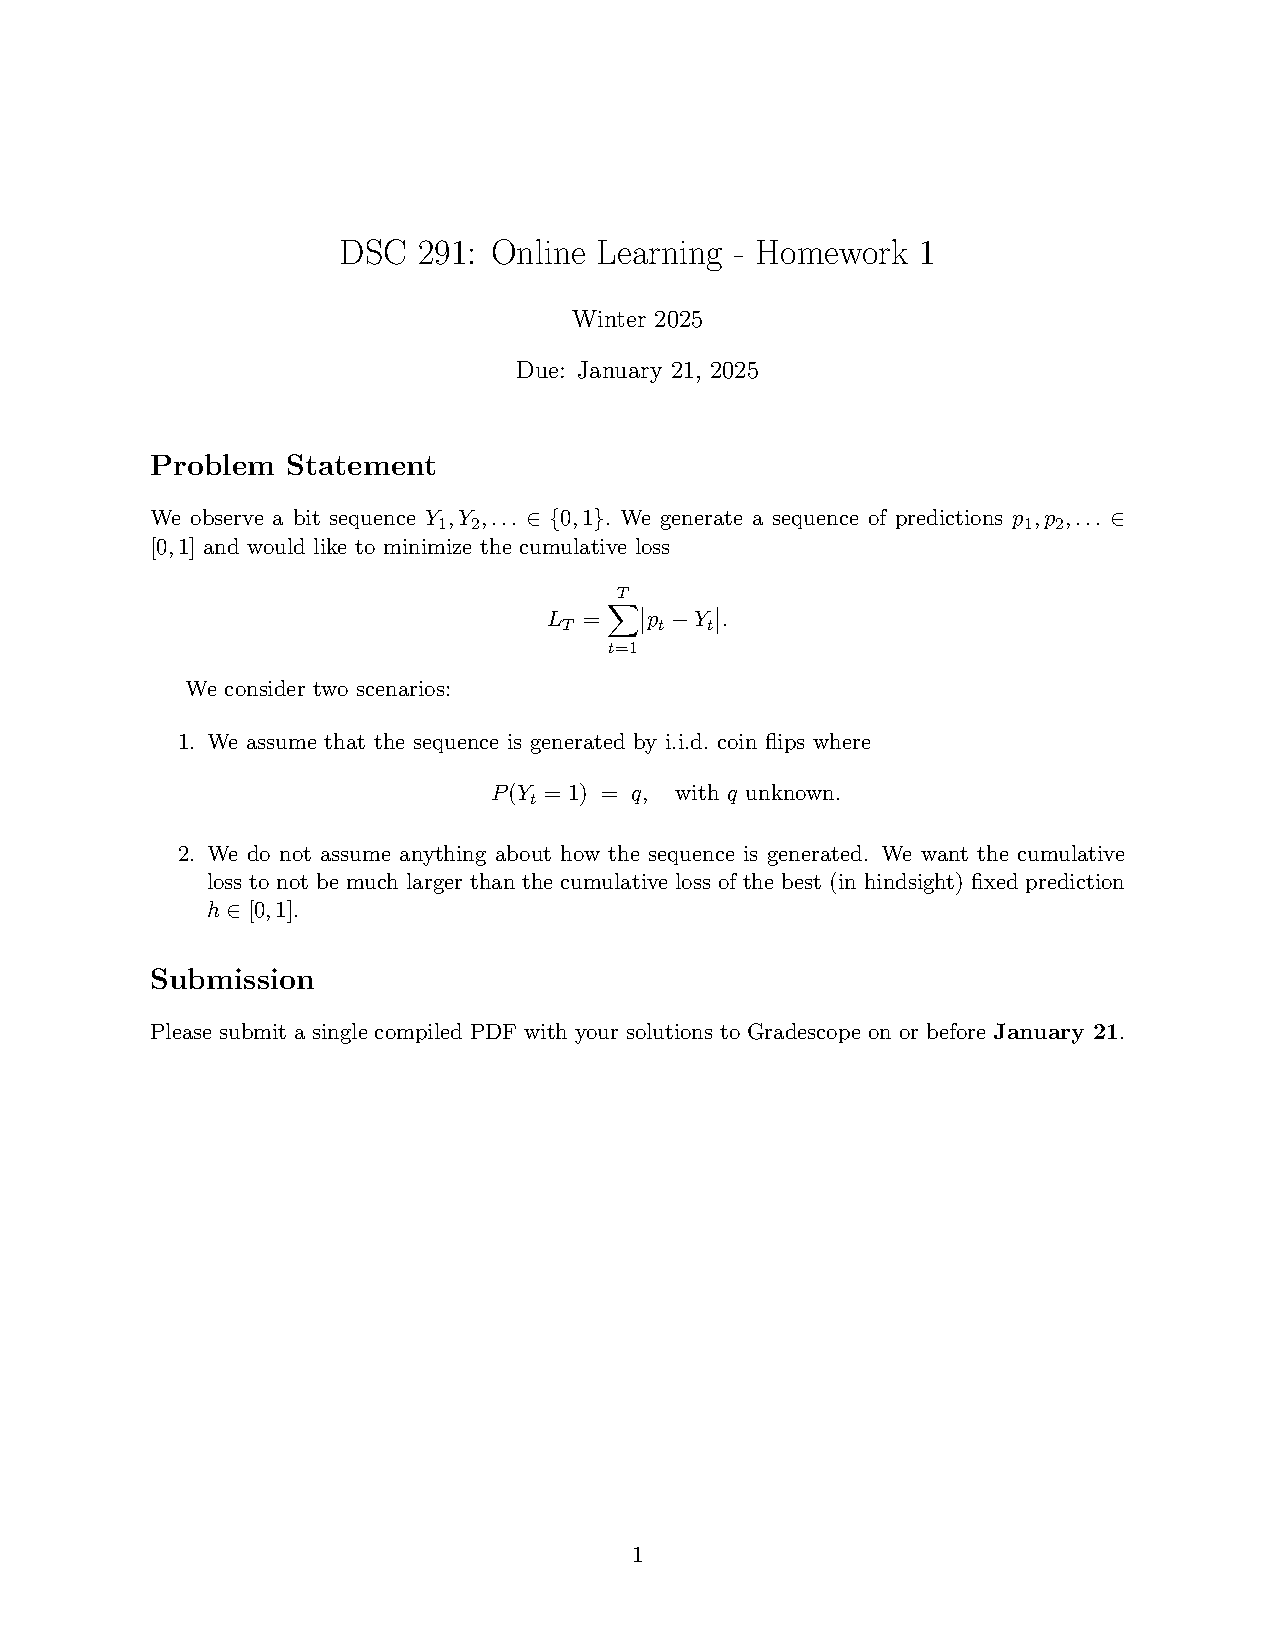
\includegraphics[width=4in]{HW1.png}
\end{itemize}
\end{frame}


\end{document}

\section{Repeated Matrix Games}

\begin{frame}
\frametitle{Zero sum games in matrix form}
\begin{itemize}
\item Game between two players.
\item Defined by \R{$n \times m$} matrix \R{$\M$}
\item \B{Row} player chooses \R{$i \in \{1,\ldots,n\}$}
\item \B{Column} player chooses \R{$j \in \{1,\ldots,m\}$}
\item \B{Row} player gains \R{$\M(i,j) \in [0,1]$}
\item \B{Column} player looses \R{$\M(i,j)$}
\item Game repeated many times.
\end{itemize}
\end{frame}

\begin{frame}
\frametitle{Pure vs. mixed strategies}
\begin{itemize}
\item Choosing a \B{single} action = \B{pure} strategy.
\item Choosing a \B{Distribution} over actions = \B{mixed} strategy.
\item \B{Row} player chooses dist. over rows \R{$\P$}
\item \B{Column} player chooses dist. over columns \R{$\Q$}
\item \B{Row} player gains \R{$\M(\P,\Q)$}.
\item \B{Column} player looses \R{$\M(\P,\Q)$}.
\end{itemize}
\end{frame}

\begin{frame}
\frametitle{Mixed strategies in matrix notation}
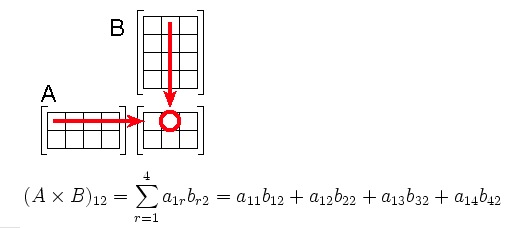
\includegraphics[width=8cm]{figures/matrixProduct.jpg}
\pause \\
\R{$\Q$} is a \B{column} vector. \R{$\P^T$} is a row vector.
%\R{$\P = \angles{ \P(1),\ldots,\P(n) }, \Q = \angles{ \Q(1),\ldots,\Q(m)}$}
\pause \\ ~\\
\R{$\M(\P,\Q) = \P^T \M \Q = \sum_{i=1}^n \sum_{j=1}^m \P(i) \M(i,j) \Q(j)$}
\end{frame}

\begin{frame}
  \frametitle{The minmax Theorem}
~\\
When using pure strategies, second player has an advantage.
~\\~\\ ~\pause
\B{John von Neumann, 1928.}
\\ ~ \\ 
\R{\[ \minp \maxq \mpq = \maxq \minp \mpq \]}
\\ ~ \\ 
In words: for \B{mixed} strategies, choosing second gives no advantage.
\end{frame}

\begin{frame}
\frametitle{Minmax is weaker than diminishing regret}
\begin{itemize}
\item The minmax theorem proves the existence of an \B{Equilibrium}.
\item Learning guarantees no regret with respect to the past.
\item If all sides use learning, then game will converge to minmax equilibrium.
\item If opponent is not optimally adversarial (limited by knowledge, computationa power...) then learning gives \B{better} performance than min-max.
\item Our goal is to minimize regret.
\end{itemize}
\end{frame}


%%% Local Variables:
%%% mode: latex
%%% TeX-master: t
%%% End:
